\documentclass[master=cws, twoside]{kulemt} \setup{title={Programmeren en
  Bewijzen met Dependently Typed Talen}, author={Toon Nolten}, promotor={Dr.\
  Dominique Devriese \and Prof.\,dr.\,ir.\ Frank Piessens},
  assessor={Prof.\,dr.\ Marc Denecker \and Dr.\ Thomas Heyman},
assistant={Jesper Cockx}}
% De volgende \setup mag verwijderd worden als geen fiche gewenst is.
\setup{filingcard, translatedtitle={Programming and Proofs in Dependently Typed
  Languages}, udc=681.3, shortabstract={In this thesis we present two case
    studies, both in Agda, a fully dependently typed programming language, and
    in Haskell, a functional programming language with a Hindley-Milner style
    type system. After formulating a model of a problem in Agda, we mimic this
    model in Haskell, relying on Glasgow Haskell Compiler extensions to provide
    type system features we lack in standard Haskell. We try to illustrate how
    much, or little effort goes into static verification. And hint at reducing
    reliance on test suites by encoding simple properties in our types.}}

% TODO: toggle voor gedrukte versie?
\usepackage[pdfusetitle,colorlinks,linkcolor=black,citecolor=black,urlcolor=black,plainpages=false]{hyperref}

\usepackage{amsmath}
\usepackage{amssymb}
\usepackage[outputdir=_build]{minted}
\usepackage{underscore}
\usepackage{subcaption}
\usepackage{import}
\usepackage{textgreek}

% Missing unicode characters for Agda
\usepackage{MnSymbol}
\DeclareUnicodeCharacter{"2237}{$\squaredots$}
\DeclareUnicodeCharacter{"25C2}{$\blacktriangleleft$}
\DeclareUnicodeCharacter{"25B8}{$\blacktriangleright$}
\DeclareUnicodeCharacter{"1D9C}{$^{c}$}
\DeclareUnicodeCharacter{"225F}{$\stackrel{?}{=}$}
\DeclareUnicodeCharacter{"25A0}{$\blacksquare$}

% More readable minted commands
\newmintinline[iagda]{agda}{}
\newmintinline[ihask]{haskell}{}

\newmintedfile[inputagda]{agda}{}
\newmintedfile[inputhaskell]{haskell}{}

\begin{document}

\begin{preface} Ik heb dit thesisonderwerp gekozen omdat ik erg geïnteresseerd
  ben in programmeertalen. Van jongs af aan heb ik me altijd afgevraagd hoe
  dingen werken. Eén van de grootste raadsels was hoe een computer nu eigenlijk
  werkt. Ik heb redelijk snel geleerd dat een computer eigenlijk niets meer is
  dan een machine die een stroom van bits omzet in een andere stroom van bits.
  Niet dat ik daarmee volledig begreep hoe een computer werkt op het niveau van
  bits en bytes, maar ik kon me er toch iets bij voorstellen. Waar bij mij het
  interessantste probleem zat was de omzetting van een programma zoals wij het
  zouden schrijven naar zo een stroom van bits. Stilaan heb ik dan geleerd wat
  een compiler is en dat bracht eigenlijk alleen meer problemen met zich mee:
  ``Hoe kan de C compiler in C geschreven zijn?'' Dit maar om aan te geven dat
  ik het een fascinerend onderwerp vind. De interesse in dependent types is
  eigenlijk eerder toevallig gekomen. Ik had de beschrijving van het onderwerp
  al eens gelezen en daarbij moest ik meteen denken aan hoe het typesysteem van
  Java mij al had tegengewerkt in vorige opdrachten. Maar ik dacht tegelijk ook
  aan Haskell wat een veel aangenamer typesysteem heeft. En die dissonantie is
  eigenlijk de reden dat ik voor dit onderwerp gekozen heb. Waarom is het ene
  typesysteem eerder aangenaam om mee te werken en het andere niet? En
  belangrijker nog: ``Hoe ver kan een typesysteem gaan?''

  Ik wil ook nog een aantal mensen bedanken. In de eerste plaats mijn
  begeleider Jesper en mijn promotor Dominique, zij hebben mij tegelijk op het
  juiste pad gezet en mij veel zelfstandigheid gegeven in wat ik juist wou doen
  en hoe ik het wou doen. Ook heb ik veel gehad aan discussies in de \#agda en
  \#haskell IRC kanalen op het freenode netwerk waarbij ik vermijd namen te
  noemen omdat de kans groot is dat ik iemand vergeet. Verder wil ik mijn vader
  bedanken die altijd bereid was te luisteren naar een al te vaak ingewikkelde
  uitleg wanneer ik me een nieuw concept probeerde eigen te maken. Natuurlijk
  kan ik niet vergeten mijn moeder te bedanken voor het rusteloze aandringen om
  nu toch eindelijk is aan die thesis te beginnen werken. Tenslotte wil ik mijn
  grootvaders bedanken die me met hun uitgebreide kennis geïnspireerd hebben om
  altijd vragen te blijven stellen.
\end{preface}

\tableofcontents*

\begin{abstract}
  Dependent types vormen een krachtig middel om bepaalde eigenschappen te
  coderen in het typesysteem. Op deze manier moeten we niet telkens aan alle
  eigenschappen proberen denken. Wat de computer voor ons kan doen, moeten we
  zelf niet doen. In programmeertalen is er al lang een tendens om meer door de
  computer zelf te laten doen, bijvoorbeeld het geheugenbeheer met garbage
  collectors. Wat typesystemen betreft is dit jammer genoeg nog niet het geval.
  Er wordt wel onderzoek verricht maar dit komt zelden terecht in een van de
  talen die voor alledaagse taken worden gebruikt. Haskell is één van de
  uitzonderingen op deze regel. Het is een taal die zijn nut in de praktijk al
  bewezen heeft. En die tegelijkertijd nog het onderwerp is van onderzoek om
  betere technieken te vinden voor onder andere typesystemen en concurrency.
  Agda staat in vergelijking nog in de kinderschoenen maar dit maakt het ook
  mogelijk om op een sneller tempo te experimenteren.

  In deze thesis proberen we aan de hand van twee gevalstudies een beter zicht
  te krijgen op programmeren met dependent types. Waarvoor het nuttig kan zijn:
  meer concepten uitdrukken op een type safe manier en statisch eigenschappen
  verifiëren bijvoorbeeld. Wat er aan schort: geen inferentie van types,
  \emph{verbose}. En hoe een taal die eigenlijk geen dependent types heeft zich
  verhoudt tot een dependently typed taal.
\end{abstract}

\mainmatter

\chapter{Inleiding}
\label{inleiding}

types
dependent types
agda
haskell
vec relalg

In deze thesis worden twee programmeertalen met een sterk typesysteem
vergeleken. Dit met een nadruk op het typesysteem van de talen eerder dan de
talen zelf. Het gaat hier om twee functionele programmeertalen: Agda
\ref{agda}, een dependently typed programmeertaal, en Haskell \ref{haskell},
een taal met een Hindley-Milner \ref{hindmil} typesysteem.


\section{Typesysteem}

Een typesysteem is een verzameling van regels waaraan code in een bepaalde
programmeertaal moet voldoen. Er zijn vershillende redenen om zulke regels op
te leggen. De belangrijkste is type safety; dit betekent dat de computer nooit
onzinnige bewerkingen zal uitvoeren, wat een onzinnige bewerking juist is,
hangt af van het typesysteem. Gewoonlijk worden bewerking zoals optelling enkel
gedefinieerd op getallen, een voorbeeld van een onzinnige bewerking zou dan een
optelling kunnen zijn van een getal en een lijst. Een andere vorm van
bescherming die onder type safety valt is memory safety. Een belangrijke vorm
hiervan is bescherming tegen buffer overflows, deze hebben vaak security
vulnerabilities tot gevolg maar als het typesysteem over genoeg informatie
beschikt, kan gegarandeerd worden dat ze niet voorkomen.

%%%%%%%%%%%%%%%%%%%%
% Chapters

\chapter{Programmeertalen}
\label{ch:agda-haskell}

In dit hoofdstuk beschrijven we de programmeertalen die gebruikt zijn in de
gevalstudies. Er moet ergens een grens getrokken worden die bepaald wat wel en
niet uitgelegd wordt, deze thesis veronderstelt dat de lezer vertrouwd is met
getypeerd functioneel programmeren.
Omdat Agda minder bekend is, is de uitleg hierover uitgebreider dan die over
Haskell. Het enige dat we voor Haskell moeten uitleggen zijn namelijk de
extensies van GHC \ref{ghc} die we gebruiken.


\section{Agda}

Agda is een dependently typed programmeertaal. Talen met dependent types zijn
dankzij de Curry-Howard correspondence ook bruikbaar als bewijsassistent. In
vele andere talen met dependent types ligt de nadruk ook eerder op het gebruik
als bewijsassistent dan wel als programmeertaal.

\subsection{Dependent Types}

Het belangrijkste verschil tussen Agda en andere functionele programmeertalen
is het typesysteem. Een dependent type is een type dat afhangt van een waarde.
De voorgaande zin legt eigenlijk alles uit dat belangrijk is aan dependent
types maar iemand die nog niet vertrouwd is met dependent types zal hier weinig
van opsteken. Vandaar overlopen we een aantal voorbeelden in Agda: eerst om de
syntax te verduidelijken, daarna om te illustreren wat dependent types nu
eigenlijk zijn.

De definitie van nieuwe types gebeurt gelijkaardig als in andere getypeerde
functionele programmeertalen. Een \iagda{data} sleutelwoord wordt gevolgd door
de naam van het type, een dubbel punt, het type van het type, dan het
sleutelwoord \iagda{where} en op de volgende regels de constructors met hun
type. Nemen we als voorbeeld een definitie voor natuurlijke getallen:

%----------------------------------------%
\begin{minted}[fontsize=\small]{agda}
  data Nat : Set where
    zero : Nat
    suc  : Nat → Nat
\end{minted}

Dit geeft ons een unaire voorstelling van de natuurlijke getallen, het getal 2
stellen we bijvoorbeeld voor als volgt: \iagda{suc (suc zero)}. Een verschil
met andere talen is dat we het type van het type moeten opgeven.  In
dependently typed talen is de scheiding tussen types en waarden fundamenteel
opgeheven. Het type van de meeste eenvoudige types is in Agda \iagda{Set}, wat
eigenlijk \iagda{Set₀} is. Het type van \iagda{Set₀} is \iagda{Set₁} en deze
hiërarchie gaat in theorie oneindig ver door. Haskell heeft gelijkaardige
concepten maar daar gaat de hiërarchie niet erg ver door. De hiërarchie gaat
als volgt in Haskell, met de Engelse termen omdat ze niet allemaal een goede
vertaling hebben: een value heeft een type, een type heeft een kind, een kind
heeft een sort en hier stopt de hiërarchie. Het dichtste equivalent van
\iagda{Set} is in Haskell het kind \ihask{*}, \ihask{*} heeft nog sort
\ihask{BOX} maar \ihask{BOX} heeft zelf sort \ihask{BOX}. Merk op dat
\ihask{BOX} enkel en alleen een intellectueel concept is, het is niet uit te
drukken in Haskell zelf.  Het tweede verschil met een type declaratie in een
taal zoals Haskell is dat we het type van elke constructor moeten opgeven, voor
\iagda{Nat} is dit heel eenvoudig. In het volgende voorbeeld wordt duidelijker
waarom we deze types moeten specificeren.

Dit voorbeeld wordt vaak gebruikt om het concept van dependent types te
illustreren. Deze code komt uit de Agda Standard Library \ref{agda:stdlib} maar
is licht aangepast om het voorbeeld eenvoudiger te maken.

%----------------------------------------%
\begin{minted}[fontsize=\small]{agda}
  data Vec (A : Set) : ℕ → Set where
    []  : Vec A zero
    _∷_ : ∀ {n} (x : A) (xs : Vec A n) → Vec A (suc n)

  head : ∀ {n} {A : Set} → Vec A (suc n) → A
  head (x ∷ xs) = x
\end{minted}

\iagda{Vec} is het type voor lijsten met een vaste lengte, vanaf nu noemen we
dit vectors. Hier zien we twee nieuwe dingen, het type \iagda{Vec} verwacht nog
twee argumenten. Het eerste is de parameter voor de dubbel punt, \iagda{A} met
als type \iagda{Set} dus \iagda{A} is een eenvoudig type. Het tweede is de
index van het type \iagda{ℕ}, dit is de naam van het type voor natuurlijke
getallen uit de standard library, het verschil tussen een index en een
parameter is dat een index voor elke constructor kan variëren terwijl een
parameter voor alle constructors hetzelfde is. Een type met indices noemen we
ook wel een inductieve familie \ref{indfam}. De lege vector, \iagda{[]},
heeft lengte nul, het type is \iagda{Vec A zero}: het is dus een vector van
elementen van type \iagda{A} met lengte \iagda{zero}. De constructor die
langere vectoren maakt, verwacht een element, \iagda{x} van type \iagda{A}, een
vector met elementen van hetzelfde type \iagda{A} en een bepaalde lengte
\iagda{n}, namelijk \iagda{xs} met als type \iagda{Vec A n}, en geeft een
vector terug waarvan de lengte één groter is, \iagda{Vec A (suc n)}. De
\iagda{head} functie, die het eerste element van een vector terug geeft kan dan
eisen dat ze enkel werkt op vectoren met een lengte groter dan nul, vectoren
met type \iagda{Vec A (suc n)}. Als de lengte niet in het type opgenomen is,
kan een functie er ook geen voorwaarden aan opleggen. Zo moet de \ihask{head}
functie voor gewone lijsten in Haskell een fout opwerpen wanneer ze opgeroepen
wordt met een lege lijst als argument.  Dit is een heel eenvoudig voorbeeld en
hieruit blijkt niet welke van de twee een betere manier is om lijsten voor te
stellen.  Het laat wel zien wat het betekent voor een type om af te hangen van
een waarde. Wat we ook zien, zowel in het type van \iagda{_∷_} als \iagda{head}
is \iagda{∀ {n}}, de universele kwantor zorgt dat \iagda{n} eender wat kan
zijn zolang het voldoet aan de eisen in de rest van het type. De accolades rond
\iagda{n} en in het type van \iagda{head} ook rond het type van het volgende
argument, \iagda{{A : Set}}, duidt aan dat deze argumenten impliciet zijn, ze
worden afgeleid uit de context, in dit geval bijvoorbeeld uit het type van het
vector argument.

Een meer uitgebreid voorbeeld uit een artikel dat het nut van dependent types
goed uitlegt \ref{TPoP}, laat zien dat dependent types zeer expressief zijn.
Het type \iagda{RA} laat toe om een relationele algebra expressie op te stellen
die correct is door constructie. Het artikel beargumenteert dat het in Haskell
niet mogelijk is om een interface naar een database te voorzien die evenveel
statische garanties biedt en even volledig - joins zijn zonder dependent types
moeilijk te typeren - is zonder gebruik te maken van preprocessing of
experimentele features. Dit betekent niet dat er geen libraries bestaan voor
Haskell die bepaalde eigenschappen statisch of dynamisch op leggen, maar wel
dat die beperkter zijn en minder statisch kunnen zijn. Statische correctheid is
handiger omdat ze geen uitvoerige testen noodzakelijk maakt.

%----------------------------------------%
\begin{minted}[fontsize=\small]{agda}
  data RA : Schema → Set where
    Read    : ∀ {s} → Handle s → RA s
    Union   : ∀ {s} → RA s → RA s → RA s
    Diff    : ∀ {s} → RA s → RA s → RA s
    Product : ∀ {s s'} → {_ : So (disjoint s s')} → RA s → RA s'
              → RA (append s s')
    Project : ∀ {s} → (s' : Schema) → {_ : So (sub s' s)} → RA s → RA s'
    Select  : ∀ {s} → Expr s BOOL → RA s → RA s
\end{minted}

Het type \iagda{Schema} stelt een schema van een relatie voor, door dit als
index op te nemen, kunnen we bepaalde eisen stellen aan de schema's waarop een
relationele expressie werkt. De \iagda{Read} constructor gelijkt een beetje op
een lege lijst omdat die aan de basis van elke relationele expressie moet
liggen, voor alle andere constructors voor een relationele expressie hebben we
al een relationele expressie nodig. \iagda{Read} bevat de informatie die
aangeeft in welke database de relatie te vinden is in een \iagda{Handle}. Zo'n
\iagda{Handle} heeft tevens een schema als index en kunnen we enkel opstellen
als de database inderdaad een relatie heeft die aan het schema voldoet. Voor de
unie van twee relaties, \iagda{Union}, en het verschil tussen twee relaties,
\iagda{Diff}, eisen we dat de schemas overeenkomen: een relatie kan maar een
unie zijn van twee relaties als alle attributen overeenkomen, eigenlijk moeten
de schema's niet hetzelfde zijn maar mogen ze permutaties van elkaar zijn maar
dit kan opgelost worden door de implementatie van \iagda{Schema}. De
constructor voor het cartesisch product, \iagda{Product}, heeft een impliciet
argument van het type \iagda{So (disjoint s s')}, de underscore duidt aan dat
we het argument niet gebruiken in de rest van het type maar moet er staan omdat
we een type van een impliciet argument niet zonder een variabele kunnen
opgeven. Het type \iagda{So (disjoint s s')} zorgt ervoor dat de schemas
\iagda{s} en \iagda{s'} disjunct zijn omdat een relatie geen twee attributen
met dezelfde naam kan hebben en een cartesisch product geen join is. Verder
zien we dat \iagda{Product} een relationele expressie opstelt waarvan het
resulterende schema de combinatie van de disjuncte schema's is. Voor de
projectie, \iagda{Project}, eisen we dat de attributen die we uit een relatie
willen projecteren inderdaad aanwezig zijn in de relatie. Het belangrijkste
kenmerk van de \iagda{Select} constructor kunnen we helaas niet uitleggen
zonder meer van het artikel over te nemen maar is niet belangrijk in de rest
van dit werk.

\subsection{Syntax}

Wat ook opmerkelijk is aan Agda, is de vrijheid die er is door de flexibele
syntax. Agda legt geen regels op in verband met hoofdletters voor types en
constructors en kleine letters voor functies, dit mes snijdt natuurlijk aan
twee kanten omdat types en functies minder gemakkelijk uit elkaar te houden
zijn. Wat waarschijnlijk de belangrijkste reden is om zulke regels niet af te
dwingen is dat er eigenlijk geen verschil is tussen waarden en types, een
functie is ook een waarde, het is dus ook niet logisch om artificieel een
verschil op te leggen in de schrijfwijze. Wat naamgeving betreft is nog een
belangrijk kenmerk dat alle unicode karakters toegelaten zijn. Hier wordt in de
standard library ook veel gebruik van gemaakt. Praktisch betekent dit dus dat
er goede ondersteuning moet zijn van de tekstverwerker en het lettertype waarin
je Agda code schrijft.

Een belangrijker kenmerk van de syntax in Agda is dat types, constructors en
functies gedefinieerd kunnen worden met mixfix notatie. Voor vectoren hebben we
al een infix constructor gezien, een tweede voorbeeld van zulke notatie is dit:

%----------------------------------------%
\begin{minted}[fontsize=\small]{agda}
  if_then_else_ : {A : Set} → Bool → A → A → A
  if true then x else y = x
  if false then x else y = y
\end{minted}

Deze functie kunnen we nu op twee manieren gebruiken. Met prefix notatie als we
de naam met underscores overnemen als volgt: \iagda{if_then_else_ true x y}. Of
zoals in de definitie in de mixfix vorm. Soms maakt dit de code gemakkelijker
leesbaar. Wat wel noodzakelijk wordt door zo'n flexibele notatie is het
veelvuldig gebruik van spaties, voor \iagda{if_then_else_} maakt dit weinig uit
want daar zijn de spaties logisch maar stel bijvoorbeeld dat dit een functie
is: \iagda{[_]}, dan moeten er spaties rond het argument, \iagda{[ x ]}, wat in
het begin vreemd aanvoelt maar nodig is omdat \iagda{[x]} een geldige naam zou
kunnen zijn voor een functie.


\section{Haskell}

Omdat we redelijk veel vergen van het typesysteem, komen we niet toe met
standaard Haskell zoals bijvoorbeeld geïmplementeerd in GHC maar hebben we een
aantal extensies nodig van GHC.

\subsection{Waarden op typeniveau}

Omdat we waarden nodig hebben op het niveau van types, wat dus eigenlijk types
zijn, en die types zelf een type moeten hebben, wat in Haskell dus een kind is,
maken we gebruik van de extensie DataKinds. Deze extensie laat ons toe om zelf
kinds te definiëren met bijhorende types door onze gewone types te promoveren
tot kinds en hun constructors te promoveren tot types. Een voorbeeld maakt dit
veel duidelijker:

%----------------------------------------%
\begin{minted}[fontsize=\small]{haskell}
  data Nat = Z | S Nat

  two :: Nat
  two = S (S Z)

  type_level_two :: S (S Z)
\end{minted}

We definiëren gewoon een type voor natuurlijke getallen en door de DataKinds
extensie wordt dit type een kind en de constructors types. Het kind \ihask{Nat}
is dus het kind van twee types namelijk \ihask{Z} en \ihask{S Nat}. De
\ihask{Nat} in \ihask{S Nat} is opnieuw het kind Nat niet het type. Omdat
dezelfde namen voor verschillende concepten af en toe verwarrend kunnen zijn en
het niet onmogelijk is dat we al een type \ihask{Z} gedefinieerd hadden, worden
types en constructors ook altijd gepromoveerd tot kinds en types die beginnen
met een apostrophe. Het type \ihask{Nat} wordt bijvoorbeeld altijd gepromoveerd
tot de kind \ihask{'Nat} en de constructor \ihask{Z} tot het type \ihask{'Z}.
Met deze extensie kunnen we dus waarden voorstellen op typeniveau waar de
extensie nog tekortschiet is dat de waarde \ihask{Z} en het type \ihask{Z}
volledig los van elkaar staan, buiten de naam. Er is ook geen waarde van het
type \ihask{Z}. In één van de volgende hoofdstukken gebruiken we een techniek
waarmee we de waarden op waardeniveau en typeniveau ongeveer kunnen verbinden.

\subsection{Inductieve families}

\subsection{multiparam, flexinst, polykinds}



\chapter{Case: Verified Koopa Troopa Movement}
\label{ch:case-koopa}


\section{Inleiding}

Deze eerste gevalstudie is geïnspireerd door de populaire Mario \ref{mario}
franchise van Nintendo \ref{nintendo}, in het bijzonder Super Mario Bros.
\ref{supmario}. Er zijn verschillende vijanden in het spel maar hier beperken
we ons tot de schildpadachtige Koopa Troopas. Zoals wel vaker voorkomt bevatten
vele van de Mariospellen zogenaamde \emph{glitches}, fouten die uitgebuit
kunnen worden om bepaalde acties uit te voeren die normaal moeilijk of
onmogelijk zijn. Zo is er bijvoorbeeld een fout met een Koopa Troopa waardoor
Mario aan het einde van het level over de vlag kan springen, dit is normaal
niet mogelijk. Deze fout, te zien in figuur \ref{koopaglitch} is eigenlijk de
precieze inspiratie van deze gevalstudie.

\begin{figure}
  \centering
  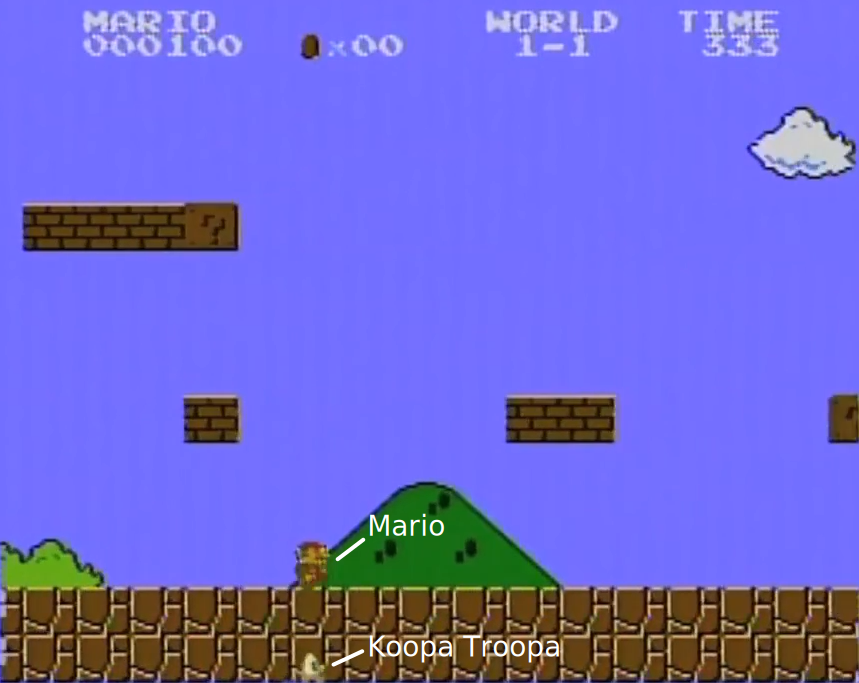
\includegraphics[width=\linewidth]{figures/KoopaTroopaGlitch}
  \caption{Onder Mario is nog net het hoofd van een Koopa Troopa te zien}
  \label{koopaglitch}
\end{figure}

De Koopa Troopas komen voor in twee kleuren: rood en groen. Ze lopen in één
richting tot ze een obstakel tegenkomen, dan keren ze om. Voor alle Koopa
Troopas is een muur een obstakel, enkel voor de rode Koopa Troopas is een
afgrond een obstakel. Dit heeft tot gevolg dat rode Koopa Troopas heen en weer
patrouilleren en groene Koopa Troopas eerder trapsgewijs naar beneden vallen
tot ze uit het beeld verdwijnen. Door deze regels uit te drukken in de types,
in plaats van in de spellogica, kunnen we een fout zoals die in figuur
\ref{koopaglitch} te zien is, voorkomen.


\section{Koopa Troopas in Agda}

Om het programmeren met dependent types zo duidelijk mogelijk te illustreren
wordt alle code stap voor stap bekeken in begrijpelijke stukken.  

De code begint met een module declaratie, deze is niet verplicht maar wel
nuttig omdat ze het mogelijk maakt de code te gebruiken in andere programma's.
Daarna importeren we een aantal eenvoudige types uit de standaard bibliotheek.

\inputagda[firstline=8, lastline=15]{agda-casestt/koopa.agda}

\iagda{Data.Nat} bevat een unaire voorstelling van natuurlijke getallen die we
gaan gebruiken voor coördinaten. \iagda{Data.Fin} definieert een type voor
begrensde natuurlijke getallen, dit gebruiken we zodat we bij index operaties
niet buiten het bereik van een lijst kunnen gaan. \iagda{Data.Vec} definieert
lijsten met een vaste lengte, vectors dus. \iagda{Data.Unit} definieert een
type, \iagda{⊤} ook wel top genoemd, met één waarde namelijk \iagda{tt}. En,
ten laatste, \iagda{Data.Empty} definieert een leeg type, \iagda{⊥} ook wel
bottom genoemd, waarvoor dus geen waarden bestaan. Dit is anders dan in Haskell
waar je eigenlijk geen leeg type kunt hebben, elk type bevat daar minstens
bottom, wat verschillende dingen kan betekenen, bijvoorbeeld niet eindiging of
een error.

Het volgende stuk is een geneste module declaratie waarin het type
\iagda{Matrix} wordt gedefinieerd als een vector van vectoren en een functie
die een element uit een \iagda{Matrix} projecteert. \iagda{Matrix} is een
inductive family zoals eerder besproken. Omdat \iagda{Matrix} hier gedefinieerd
is als een vector van vectoren kunnen we voor de \iagda{lookup} functie de
\iagda{lookup} functies voor vectoren gebruiken. De volgorde van de indices
speelt hierbij een rol maar omdat de indices van het type \iagda{Fin n}
zijn, kan Agda een fout geven als we ze omwisselen. Vervolgens wordt de module
geopend zodat we het type en de functie kunnen gebruiken zonder de namen te
moeten kwalificeren met de naam van de module.

\inputagda[firstline=17, lastline=23]{agda-casestt/koopa.agda}

Hierna begint de oplossing van het probleem eigenlijk pas echt. We definiëren
een aantal types waarmee we de Koopa Troopas en de levels kunnen voorstellen.

\inputagda[firstline=25, lastline=30]{agda-casestt/koopa.agda}

Koopa Troopas kunnen twee kleuren hebben dus we definiëren een type
\iagda{Color} met een constructor voor elke kleur. Agda laat ons toe om
constructors met hetzelfde type te groeperen als volgt: \iagda{Green Red :
Color}. Het type \iagda{KoopaTroopa} is geïndexeerd op \iagda{Color}, dit wil
dus zeggen dat er een type is voor elke \iagda{Color}. De Constructor maakt
gebruik van de Agda syntax voor mixfix notatie, in dit geval is \iagda{KT} dus
een postfix constructor. De \iagda{_KT} constructor verwacht een
\iagda{Color} en maakt dan een waarde van het type \iagda{KoopaTroopa c} waar
die \iagda{c} dus de waarde van het argument is. Een groene Koopa Troopa kunnen
we dus voorstellen als \iagda{Green KT} en heeft het type \iagda{KoopaTroopa
Green}, later wordt duidelijk waarom het belangrijk is dat de kleur in het type
zit.

Het volgende stuk bevat nog een aantal type declaraties. Hier definiëren we
posities met alle informatie die we later nodig hebben om te bepalen op welke
posities een Koopa Troopa mag staan.

\inputagda[firstline=32, lastline=48]{agda-casestt/koopa.agda}

Elke positie is ofwel lucht ofwel vast: grond of muur of iets dergelijks. Het
type \iagda{Material} stelt deze toestanden voor. Het type \iagda{Clearance}
gebruiken we om te bepalen wie of wat waar mag komen. Een positie met
\iagda{Clearance} \iagda{Low} kan door eender welke Koopa Troopa betreden
worden maar een positie met \iagda{Clearance} \iagda{High} kan enkel door
groene Koopa Troopas betreden worden en gebruiken we om posities aan te duiden
waar de enige logische beweging vallen is. De \iagda{Clearance}
\iagda{Ultimate} gebruiken we voor posities waar geen enkele Koopa Troopa mag
komen. Een positie stellen we voor door een record met twee velden voor een
horizontale en een verticale coördinaat, een veld dat het \iagda{Material} van
de positie aangeeft en een veld voor de \iagda{Clearance}. De constructor
\iagda{pos} kunnen we gebruiken om een positie op te stellen, een voorbeeld van
een positie kan dus zijn: \iagda{pos 3 5 gas Low}, let hierbij op dat de
cijfers door Agda begrepen worden als natuurlijke getallen, hiermee kunnen we
ook enkel natuurlijke getallen voorstellen.

Om de Koopa Troopas een \iagda{Clearance} te geven moeten we ze op een of
andere manier differentiëren en het enige dat verschilt tussen de Koopa Troopas
is hun kleur wat dus de meest logische bepalende factor van de
\iagda{Clearance} wordt.

\inputagda[firstline=50, lastline=52]{agda-casestt/koopa.agda}

In plaats van groen en rood gelijk te stellen aan respectievelijk een hoge en
een lage \iagda{Clearance}, werkt de constructor \iagda{<red>} voor beide
kleuren terwijl \iagda{<green>} enkel voor groen werkt. Dit zorgt ervoor dat we
later niet moeten zorgen dat overal waar een lage \iagda{Clearance} toegelaten
is ook een hoge \iagda{Clearance} toegelaten is, een groene Koopa Troopa krijgt
gewoon de \iagda{Clearance} die hij nodig heeft. We zien hier ook dat de mixfix
notatie even goed voor types te gebruiken is, in dit geval gebruiken we dit om
het type voor te stellen als een pijl, \iagda{_c>_}, van een kleur naar een
\iagda{Clearance}.

De volgende twee definities zijn eigenlijk het belangrijkste deel van de
oplossing en steunen op alle voorgaande concepten.

\inputagda[firstline=54, lastline=61]{agda-casestt/koopa.agda}

Het \iagda{_follows_⟨_⟩} type is op het eerste zicht waarschijnlijk een beetje
vreemd, dit is omdat de waarden van het type eigenlijk minder belangrijk zijn
dan het type zelf. Het type drukt uit welke positie kan volgen op welke positie
rekening houdend met een kleur. Omdat hier de types van de constructors
belangrijk zijn, overlopen we ze een voor een. \iagda{stay} drukt uit dat een
Koopa Troopa altijd kan blijven staan zolang hij in lucht staat met een lage
\iagda{Clearance}. De \iagda{Material} moet \iagda{gas} zijn omdat een Koopa
Troopa niet in grond of muren mag staan en de \iagda{Clearance} moet
\iagda{Low} zijn omdat we willen dat ook rode Koopa Troopas kunnen stilstaan.
Eigenlijk is stilstaan niet echt een nodige \emph{beweging} maar hiermee kunnen
we later de eindpositie van een pad expliciet maken. De volgende twee
constructors \iagda{next} en \iagda{back} bekijken we tegelijk omdat ze heel
gelijkaardig zijn. Ze drukken uit dat een positie met een bepaalde
\iagda{Clearance} enkel kan volgen op een horizontaal vorige, respectievelijk
volgende, positie als de kleur van de Koopa Troopa die \iagda{Clearance}
oplevert. Ook moet de voorgaande positie een lage \iagda{Clearance} hebben, dit
is omdat we de hoge \iagda{Clearance} gebruiken voor posities waar de enige
mogelijke beweging vallen is. Het \iagda{Material} voor de posities moet nog
steeds \iagda{gas} zijn omdat Koopa Troopas niet in muren kunnen lopen.  De
laatste constructor is \iagda{fall} en die kan enkel gebruikt worden als
beweging van een positie met een hoge \iagda{Clearance}. Aangezien enkel groene
Koopa Troopas op een positie met een hoge \iagda{Clearance} kunnen geraken,
zijn dat ook de enige die kunnen vallen. Nogmaals kunnen we alleen vallen van
een positie in lucht naar een positie in lucht, Koopa Troopas kunnen dus niet
de grond in vallen.

\inputagda[firstline=64, lastline=69]{agda-casestt/koopa.agda}

Het type waarmee we de paden voorstellen die Koopa Troopas kunnen afleggen,
\iagda{Path}, moet ervoor zorgen dat enkel geldige paden worden opgesteld voor
een bepaalde Koopa Troopa. De parameter voor de kleur is impliciet omdat die
volgt uit het type van de Koopa Troopa, verder hangt de geldigheid van een pad
af van de Koopa Troopa en kan een pad maar voor één Koopa Troopa tegelijk
opgesteld worden dus is er een parameter waar we een Koopa Troopa verwachten.
Een pad gaat van een beginpositie naar een eindpositie en die moeten kunnen
variëren voor de verschillende constructors dus dat zijn indices. De
constructor voor een leeg pad, \iagda{[]}, moet een begin- en een eindpositie
hebben maar die kunnen we impliciet verkrijgen uit de vorige positie van het
pad en als er geen vorige positie is uit het verwachte type op de plaats waar
we de constructor gebruiken. De constructor om langere paden op te stellen
maakt weer gebruik van mixfix notatie, de \iagda{infixr} declaratie zorgt
ervoor dat de constructor rechts associatief is waardoor we minder haakjes
zullen nodig hebben. De constructor verwacht een positie \iagda{p}, een pad van
\iagda{q} naar \iagda{r}, \iagda{qs}, en een bewijs dat \iagda{q} kan volgen op
\iagda{p} voor de kleur van de Koopa Troopa en resulteert in een pad van
\iagda{p} naar \iagda{r}. \iagda{_↠⟨_⟩_} behoudt de geldigheid van een pad door
het argument van het type \iagda{_follows_⟨_⟩} en de enige manier om een pad te
beginnen is met een leeg pad dat sowieso geldig is. Door deze eigenschappen
zijn alle paden geldig bij wijze van constructie.

We kunnen nu paden beginnen opstellen maar een belangrijk probleem is nog dat
de geldigheid van de paden afhangt van een goede bepaling van de
\iagda{Clearance} van elke positie. Wat volgt is eerst een klein voorbeeld van
een pad en daarna een mogelijke oplossing voor een juiste bepaling van de
\iagda{Clearance} voor elke positie.

\inputagda[firstline=71, lastline=74]{agda-casestt/koopa.agda}

Om ervoor te zorgen dat de \iagda{Clearance} juist bepaald wordt, gaan we
een functie gebruiken die de regels voor de bepaling van de \iagda{Clearance}
van een positie uitdrukt.

\inputagda[firstline=78, lastline=86]{agda-casestt/koopa.agda}

De \iagda{matterToPosVec} functie verwacht twee vectoren van dezelfde lengte
met \iagda{Material}s in en twee coördinaten die aangeven bij welke positie het
eerste \iagda{Material} in de eerste vector hoort. Het resultaat is een vector
van dezelfde lengte met posities in met de juiste coördinaten, de
\iagda{Material}s uit de eerste vector en de juiste \iagda{Clearance} die
afhangt van het \iagda{Material} van de positie onder een positie, vandaar dat
we twee vectoren in de invoer nodig hebben. Het basisgeval is wanneer de
vectoren leeg zijn, in het andere geval bepaalt de functie \iagda{clearance}
wat de juiste \iagda{Clearance} voor de positie is aan de hand van het
\iagda{Material} van de positie zelf en van de positie er onder. Lucht boven
lucht heeft \iagda{Clearance} \iagda{High} omdat daar alleen gevallen kan
worden, lucht boven grond heeft \iagda{Clearance} \iagda{Low} omdat elke Koopa
Troopa moet kunnen staan. Alle grond en muur posities hebben \iagda{Clearance}
\iagda{Ultimate} omdat geen enkele Koopa Troopa zich in een muur of in de grond
mag bevinden.

Door vectoren te geven van alle \iagda{Material}s op een horizontale rij en de
rij daaronder kunnen we nu de \iagda{Clearance}s juist bepalen. Voor de
voorstelling van een level kunnen we dus een vector van zulke vectoren
gebruiken. Uiteindelijk willen we een matrix van posities die het level
voorstelt maar omdat het voor de recursie beter uitkomt als we met een vector
van vectoren werken voor de invoer, gebruiken we geen matrix voor de invoer.

\inputagda[firstline=88, lastline=98]{agda-casestt/koopa.agda}

De functie \iagda{matterToPosVecs} maakt gebruik van de vorige functie om een
vector van vectoren van \iagda{Material}s om te zetten in een vector van
vectoren van posities. Het basisgeval is de lege vector en die wordt omgezet in
een lege vector. In het recursieve geval zien we dat de \iagda{_∷_} constructor
voor vectoren gebruikt wordt in de prefix vorm, dit is omdat we willen pattern
matchen op een derde impliciet argument en drie argumenten gaan niet goed samen
met een binaire infix constructor. We gebruiken \iagda{matterToPosVec} op de
eerste vector in de vector van vectoren en op de vector daaronder, die we
verkrijgen uit de functie \iagda{unders}. \iagda{unders} is eigenlijk heel
gelijkaardig aan de \iagda{head} functie maar is specifieker voor een vector
van vectoren en heeft een \emph{fallback} argument dat we teruggeven als we de
rij onder de laatste rij nodig hebben. Het enige dat dan nog rest is om de
recursieve oproep te doen op de rest van de vector van vectoren. De
\iagda{matsToMat} functie maakt van de vector van vectoren van posities, die we
terugkrijgen uit \iagda{matterToPosVecs}, een matrix waarbij de rijen eerst van
volgorde gewisseld worden omdat de index $(0,0)$ bij een matrix linksboven zit
en in de levelvoorstelling links onder.

Met deze functies kunnen we gemakkelijk een level opstellen door de juiste
\iagda{Material}s in de juiste volgorde op te geven, hierbij wordt dan meteen
de juiste \iagda{Clearance} bepaalt voor elke positie. Om onze notatie iets
visueler te maken definiëren we nog twee functies met een unicode symbool.

\inputagda[firstline=100, lastline=114]{agda-casestt/koopa.agda}

De functies \iagda{□_} en \iagda{■_} zijn gewoon afkortingen voor
respectievelijk een vector die begint met \iagda{gas} en nog een staart
verwacht en een vector die begint met \iagda{solid} en nog een staart verwacht.
Deze functies zijn gedefinieerd met een underscore terwijl ze toch gewoon prefix
functies zijn omdat de \iagda{infixr} declaratie enkel van toepassing is op
mixfix functies. Zoals we kunnen zien is het level redelijk herkenbaar ook al
werken we eigenlijk gewoon met tekst, dit is een voordeel van werken met de
volledige unicode karakterset.

TODO figures van de koopa troopa paden

\chapter{Case: Verified Red-Black Trees}
\label{case:rbtree}


% Chapters
%%%%%%%%%%%%%%%%%%%%
\chapter{Besluit}
\label{besluit}

Dependent types zijn expressief en kunnen vele eigenschappen die we anders
ongezegd laten, duidelijk en correct formaliseren zonder veel moeite. De
afweging tussen moeite en statische garanties verdwijnt zeker niet maar is well
redelijk flexibel te bepalen. Gewoon met vectoren werken in plaats van lijsten
kost eigenlijk geen moeite en kan wel al mooie eigenschappen opleveren.
Uiteindelijk moet de afweging voorlopig nog vaak gemaakt worden op basis van
ervaring. Dependent types zijn nog niet zolang terug te vinden in \emph{echte}
programmeertalen en er zijn daardoor nog geen regels die we kunnen volgen over
hoeveel statische verificatie het grootste voordeel biedt tegenover de kleinste
inspanning. 

Wat we ook gezien hebben is dat, ook al zijn talen met dependent types nog niet
klaar voor algemeen gebruik, de ideeën die we erin opdoen gedeeltelijk
toepasbaar zijn in een taal zoals Haskell. Leren programmeren met dependent
types is dus geen tijdverspilling. Het heeft een dieper inzicht in het gebruik
van types in andere talen tot gevolg. En de technieken kunnen af en toe ook
overgezet worden naar die talen. 

De gevalstudies hebben laten zien dat bepaalde concepten helemaal niet moeilijk
te formaliseren zijn met dependent types. En dat door redelijk eenvoudige
formalisaties toch redelijk wat fouten kunnen worden voorkomen. We hebben ook
gezien dat Haskell redelijk ver te drijven is naar het dependently typed
programmeren, ook al wordt het steeds lastiger hoe dichter we bij dependent
types proberen komen. Hoewel ontwikkelingen zoals het singleton package voor
verbetering kunnen zorgen. Wat misschien nog de belangrijkste conclusie uit de
gevalstudies is, is dat als we een kleine toegeving doen op de precisie van de
types, we af en toe een grote vermindering van inspanning kunnen krijgen. En,
zolang de meeste eigenschappen nog in het typesysteem uitgedrukt zijn, kunnen
we die uit ons hoofd zetten en nadenken over belangrijkere problemen.

Alle code die besproken is, is beschikbaar in de bijlagen alsook op het
internet \url{https://github.com/toonn/pbdtt}.


\appendixpage*
\appendix
%%%%%%%%%%%%%%%%%%%%
% Appendices
\chapter{KoopaTroopas in Agda}
  \label{app:case-koopa-agda}
  \inputagda[fontsize=\small, breaklines]{agda-casestt/koopa.agda}

\chapter{KoopaTroopas in Haskell}
  \label{app:case-koopa-haskell}
  \inputhaskell[fontsize=\small, breaklines]{haskell-casestt/koopa.hs}

\chapter{Red-Black Trees in Agda}
  Eerst volgt een redelijk letterlijke vertaling van de code van Okasaki naar
  Agda om te tonen dat dependent types absoluut niet verplicht zijn. Daarna de
  code van de tweede case in Agda.
  \section{Okasaki}
  \inputagda[fontsize=\small, breaklines]{agda-casestt/Okasaki.agda}
  \section{Red-Black Trees}
  \label{app:case-rbtree-agda}
  \inputagda[fontsize=\small, breaklines]{agda-casestt/RedBlackTree.agda}

\chapter{Red-Black Trees in Haskell}
  Eerst volgt de code van Okasaki dan de code voor de case en daarna nog een
  korte vertaling van de \iagda{if_the_else_} functie in Agda naar een functie
  op typeniveau in Haskell.
  \section{Okasaki}
  \inputhaskell[fontsize=\small, breaklines]{haskell-casestt/Okasaki.hs}
  \section{Red-Black Trees}
  \label{app:case-rbtree-haskell}
  \inputhaskell[fontsize=\small, breaklines]{haskell-casestt/RedBlackTree.hs}
  \section{Type Level If}
  \inputhaskell[fontsize=\small, breaklines]{haskell-casestt/if.hs}
% Appendices
%%%%%%%%%%%%%%%%%%%%

\backmatter

%%%%%%%%%%%%%%%%%%%%
% References
% Je kan de  standaard "abbrv" bibliografiestijl vervangen door een andere.
\bibliographystyle{IEEEtran}
\bibliography{referenties}
% References
%%%%%%%%%%%%%%%%%%%%

\end{document}
